\chapter{Controller Development}
\label{chap:Controller Development}

\section{Active Compliance}

Passive compliance consists of using mechanical spring-damper components to adjust the dynamics of a robotics end effector. These come in the form of torsional springs, linear springs, hydraulic and pneumatic dampers to name a few. 

In the study by G.A. Pratt and M.M. Williamson  passive compliance in the form of a Series Elastic Actuator (SEA) was said to provide shock tolerance, lower reflected 
inertia, more accurate and stable force control, less damage to the environment, and the capacity for energy storage.\cite{Pratt1995}

Active compliance (AC) in robotic platforms is a relatively new area of research. Active compliance was chosen instead of passive compliance (PC) for the following reasons:

\begin{enumerate}
\item AC is mechanically simpler.
\item AC is mechanically lighter.
\item Good PC is expensive to implement due to lack of application specific off-the-shelf parts.
\end{enumerate}

Most importantly, AC can be configured on the fly to adapt to the environment of the robot. This allows a robot to, much like their biological equivalents, comply to the environment based on various sensory inputs, or to perform various acrobatic tasks making use of spring-damper compression and decompression.

Various combinations of AC spring-damper configurations were designed, implemented and tested in order to determine the best topology.

A high level controller was used to switch between the active compliance models during phase transitions as developed in \cref{sec:Control Loop Design} and seen in \cref{fig:phase-transitions}.

\section{Dynamic Stability}

Stand still, look around, turn around - these apparently simple tasks are composed of a network of biologically advanced sensors and muscular motor movements that seem intuitive. To do the same relatively static and stable movement with a physically free robot is complex. 

The alternative to static stability is dynamic stability. Much like a spinning top remains stable due to gyroscopic effects when a stationary top topples over; a dynamically hopping leg remains upright with a relatively simple control system compared to a leg trying to remain upright and walk forward.

In the book by  M.H. Raibert et al., \textit{Legged Robots That Balance}, an easily adaptable simple control algorithm for dynamic legged hopping was published. Raibert showed that complex robots can be dynamically stable, but when at rest this is more difficult. For this reason the control algorithm used for Baleka relies on the fact that Baleka is constrained in a single axis. Control of Baleka in the vertical axis will be implemented during jumping.

\section{Mechanical Impedance}
The leg design has inherent mechanical impedance in the form of friction, slack and inertial mass. Without mechanical impedance the leg would continue acting like an ideal system when actuated. This can be seen in \cref{sec:Virtual Spring-damper Tests} where the leg is modelled as a spring-damper - the amplitude of the oscillation of the virtual spring model with spring constant $K_s = 100\ N/m$ and no damping decays with time, confirming mechanical impedance. 

This mechanical impedance is not easily accounted for in the dynamic model of the leg as it is highly non-linear in the case of a complex linkage system as used in the Baleka leg - this makes it difficult to control. The mechanical impedance was treated as a disturbance and in the case of dynamic movement of the leg it was ignored. Energy will be lost in the hopping motion and during leg movement, but this is insignificant and only noticeable when doing spring-damper tests as seen in \cref{fig:spring-damper-tests}.

\section{Control Loop Sampling Frequency}

For high bandwidth proprioceptive force control S. Kalouche showed that the control loop sampling frequency should ideally be in the $kHz$ scale.\cite{Kalouche2016} This allows the foot force to ideally match the expected foot force when performing high frequency dynamic movements. 

The control loop sampling frequency was practically limited by the motor driver response time as seen in \cref{fig:packet-timing}. For every packet sent to the motor driver a response is required before the next packet can be sent otherwise the driver system becomes unstable. A maximum stable sampling frequency of $200 Hz$ was achieved with room for packet decoding, processing and controller action.

During the jump tests in \cref{sec:Jump Test} the limitations of a low sampling frequency were seen. Highly dynamic manoeuvres had a duration of approximately $20\ ms$ and this left 4 sample points for the controller to act.

\section{Force Control}
\label{sec:Force Control}

Using the virtual model developed in \cref{chap:Dynamic Modelling} we need to take the polar spring damper force and map it to the Baleka two degree of freedom system where the motors provide the needed torque.

The forward kinematic Jacobian developed in \cref{chap:kinematics} is used to determine what the motor torques are for specific $r$ and $s$ force components, where $F_r$ and $F_s$ are the components of the foot force vector. In order to calculate the virtual model foot force components, $F_r$ and $F_s$, we use the method developed in \cref{sec:Virtual Compliance Model}.

The general Euler-Lagrange dynamic equation used in \cite{Patel2015} can be further simplified for the virtual model force control problem:

\begin{equation} \label{eq:dynamic-eq}
M\ddot{q} + C\dot{q} + G = B \tau_m + Q + A^T F
\end{equation}

Assuming we can ignore centrifugal and Coriolis forces, $C$, as well as gravitational forces, $G$. The generalized force vector, $Q$, will be ignored for simplicity - comprising all disturbances and friction. Disturbances and friction will be accounted for during foot force calibration, under the assumption of a constant frictional force and miscellaneous disturbances during motion. 

Assuming both motors contribute to the end effector force equally, we can make the input mapping matrix $B$ the identity matrix.

Taking the Jacobian of the kinematic mapping $f(\phi_1, \phi_2)$ the foot force vector, F, can be transformed to the motor torque commands, $\tau$ using \cref{eq:dynamic-eq} as follows:

\begin{equation}
\tau_m = J^TF
\end{equation}

Substituting for the Jacobian and force vectors:

\begin{equation} \label{eq:motor-torques}
\begin{aligned}
& \tau_{m_1} = J^T_{11}\times F_r + J^T_{12}\times F_s \\
& \tau_{m_2} = J^T_{21}\times F_r + J^T_{22}\times F_s \\
\end{aligned}
\end{equation}

The motor current needed to produce the resulting motor torques in \cref{eq:motor-torques} is then calculated as further discussed in \cref{sec:Current Control}.

\subsubsection{Motor Torque Predictions}
\label{sec:Motor Torque Predictions}

Using a virtual model compliance model with a spring force of $K_s = 250\ N/m$ on both the radial and rotational leg polar coordinates, the motor torque predications were simulated over the kinematic workspace for each motor. \Cref{fig:Radial and rotational spring foot force mapping to motor torque} shows the motor torque plots for full leg compliance control and \cref{fig:Radial and rotational spring foot force mapping to motor torque} uses purely a torsional spring.

The data analysis shows that a higher motor torque is needed to implement a torsional spring based on the arc-length measure than the radian measure, as developed in \cref{sec:Torsional Spring-damper}. When the leg is displaced rotationally, the motor on the opposite side to the rotation develops the most torque to try and correct the error. The motors clearly develop more torque for a rotational offset than for a radial offset, as shown by the heat map hot spots on the edges of the plot.

\begin{figure}
\centering
\subfloat[][$K_s = 250$, $K_d = 0$, using arc-length measure.]{
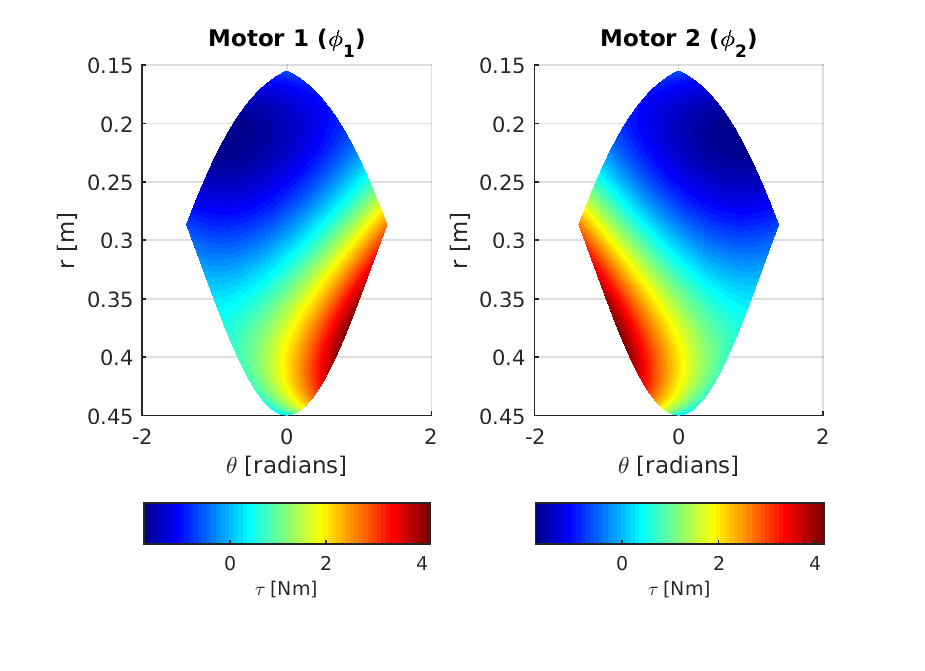
\includegraphics[width=0.8\textwidth]{images/control/forward-kinematic-motor-torque-s-0.eps} 
}

\subfloat[][$K_s = 250$, $K_d = 0$, using radian measure.]{
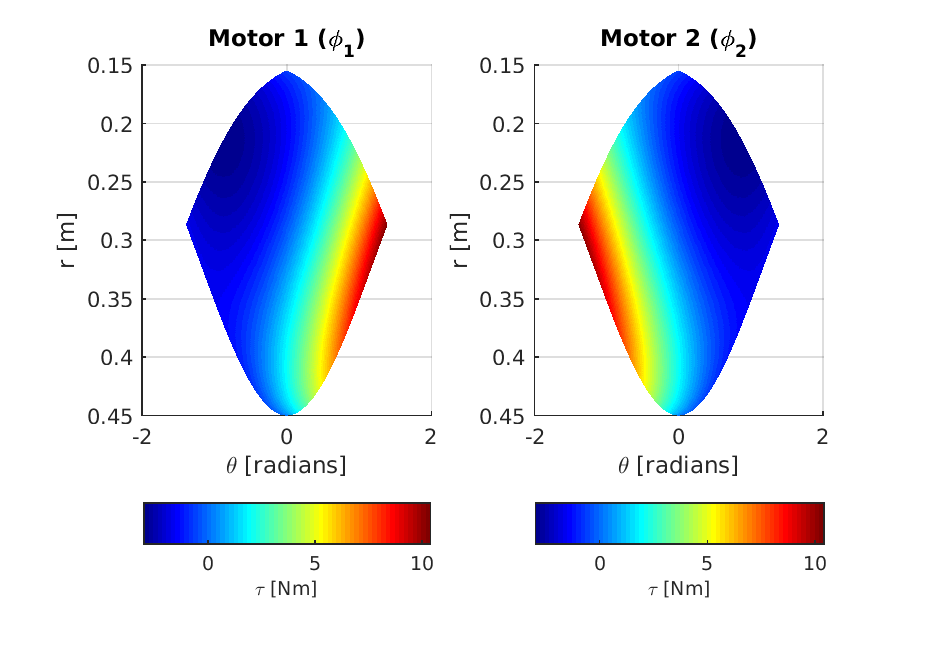
\includegraphics[width=0.8\textwidth]{images/control/forward-kinematic-motor-torque-theta-0.eps} 
}
\caption{Radial and rotational spring foot force mapping to motor torque.}
\label{fig:Radial and rotational spring foot force mapping to motor torque}
\end{figure}

\begin{figure}
\centering
\subfloat[][$K_s = 250$, $K_d = 0$, using arc-length measure.]{
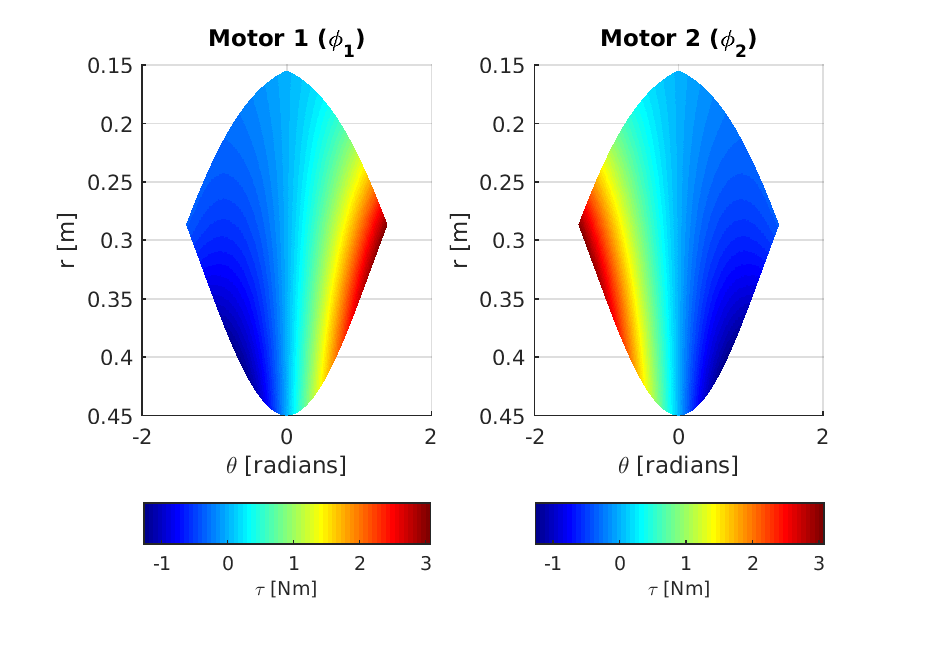
\includegraphics[width=0.8\textwidth]{images/control/forward-kinematic-motor-torque-s-only-0.eps} 
}

\subfloat[][$K_s = 250$, $K_d = 0$, using radian measure.]{
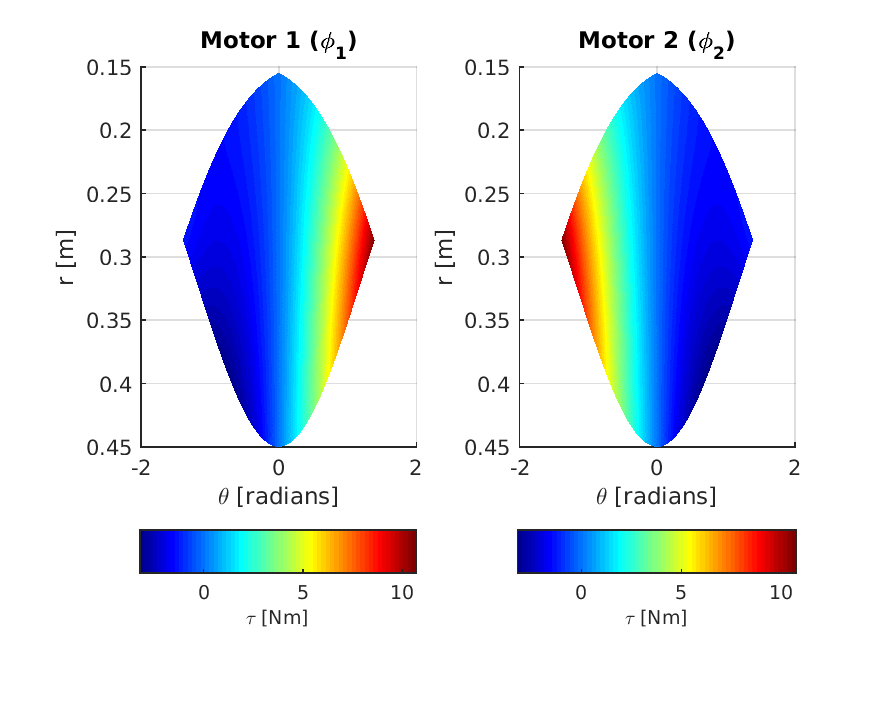
\includegraphics[width=0.8\textwidth]{images/control/forward-kinematic-motor-torque-theta-only-0.eps} 
}
\caption{Rotational spring foot force mapping to motor torque.}
\label{fig:Rotational spring foot force mapping to motor torque}
\end{figure}

\subsection{Non-conservative Forces}

In further study the non conservative forces could be determined and accounted for, but a key to virtual model control is to allow the system dynamics to naturally occur, as discussed in \cite{Pratt2001}, and the virtual components are effectively transposed on this response. If inverse dynamics are used to effectively cancel the non-conservative forces, then the system can become unstable. 

The beauty of virtual model control is in its simplicity. For the particular case of dynamic movement and jumping, the external forces can be allowed to take place and the virtual model components can be adjusted according to non-exact specifications. If on the other hand the system needs to perform precise manoeuvres, for example during robotic surgery, you'd want to be able to predict the non-conservative forces and account for them accurately.

\subsection{Current Control}
\label{sec:Current Control}

The specific motor current requirements for force control were determined in the simulation in \cref{fig:motor-current-requirements}. A maximum current of $52.3\ A$ was simulated and $60\ A$ motor drivers were selected. 

The torque constant $K_t$ was experimentally calculated in \cref{sec:Motor Model Calculations} and determined to be $0.08\ Nm/A$. Using \cref{eq:motor-torques} we can calculate the motor torque required to produce the necessary virtual model foot force. This foot force can then be mapped to a current command using the ideal linear relationship between motor torque and current:

\begin{equation}
\tau_m = \frac{1}{K_t} J^TF
\end{equation}

It must be noted that in the implementation on the embedded system it took some experimenting to determine the correct current polarity for each motor. 

During testing the current saturated at $60\ A$ during jumping. This effectively means the necessary impulsive force needed to jump to a set height was not delivered. At lower height jumps, with less current saturation, it was possible to better control the height.

Current limits in the embedded system control loop were set to just under the peak motor driver current in order to avoid current cut-out. During further testing, current cut-outs were not avoidable due to the continuous current limit of $30\ A$. In \cref{app:Jump Experiment} an example of a current cut-out during a jump is shown.

\subsection{Calibration} 

Using a load cell the value for $K_t$ was calculated in \cref{sec:Experimental Calculation of Kt} and the experiment performed in \cref{sec:Force Control Calibration and Fidelity}. By iteratively adjusting $K_t$ until the force output matched the commanded force, we can accurately control the motor torques with the appropriate current command.

\section{Control Loop Design}
\label{sec:Control Loop Design}

\Cref{fig:virtual-model-impedance-loop} is an adaptation of the control loop design found in \cite{Kalouche2016}. In \cite{Kalouche2016} continuous position loop gain scheduling is used to implement force control, whereas Baleka uses virtual spring-damper gain scheduling. This means that instead of using a position control loop and changing the gain to achieve the appropriate force, the force is changed by directly changing the virtual model spring constants. 

Borrowing from Raibert type controllers the jumping action can be split into phases, each with their own dynamic properties. These phases, and the transition between them, can be seen in \cref{fig:phase-transitions} as developed for Baleka.

At each phase transition a high level finite state machine switches between appropriate virtual model configurations. In the control loop, \cref{fig:virtual-model-impedance-loop}, these transitions are triggered by the radial position of the leg. The three specific control algorithms are for flight, launch and stance control.

The integral error action of the control loop ensures that there is zero steady state error. The rest of the control loop blocks implement the theory developed in the dynamic modelling section, \cref{chap:Dynamic Modelling}, and the force control section, \cref{sec:Force Control}.

The only part of the control loop that is left to the motor controller is the current control loop, which implements a PI controller. The motor controller gains were configured in \cref{sec:Driver Configuration}.

\begin{figure}
\centering
\includegraphics[width=0.4\textwidth]{images/control/phase-transitions.pdf} 
\caption{Jump phase transitions.}
\label{fig:phase-transitions}
\end{figure}

\begin{figure}
\centering
\includegraphics[clip, trim=2cm 8cm 5cm 3cm, page = 1, width=1\textwidth]{images/control/virtual-model-impedance.pdf} 
\caption{Virtual model impedance control loop.}
\label{fig:virtual-model-impedance-loop}
\end{figure}

\section{Torsional Spring-damper}
\label{sec:Torsional Spring-damper}

\subsection{Force Normalisation}

In previous studies using controllers for legs of similar topology, such as those by Duperret et al \cite{Duperret} and Kalouche \cite{Kalouche2016}, Cartesian coordinate systems have been used for virtual model compliance control in the case of \cite{Kalouche2016} and in the case of \cite{Duperret} a Raibert type controller was used with a polar coordinate system.

The study by Kalouche \cite{Kalouche2016} used a convenient coordinate system that had all axis of foot force and placement control in the same unit of measurement, namely distance in meters. 

By using a polar coordinate system, virtual model compliance control is made more intuitive as further developed in \cref{chap:kinematics} and \cref{chap:Dynamic Modelling}. 

The drawback to the classic polar coordinate system is the different units of measurement for radial $[m]$ and angular $[radians]$ measure. When applying torsional spring-damper dynamics to the model via control this results in vastly disproportionate force vectors that when mapped to motor torques via the Jacobian, derived in \cref{chap:kinematics}, result in an unstable control system unless the foot force components are properly scaled. 

An elegant solution to this problem and a way to normalise the angular foot force component is to use the relation in \cref{eq:arc-length-mapping} and visualised in \cref{fig:Arc-length vs. radian measure geometry}.

\begin{equation} \label{eq:arc-length-mapping}
s = r \theta
\end{equation}

\begin{figure}
\centering
\includegraphics[clip, trim=2cm 8cm 2cm 2cm, page=1, width=0.5\textwidth]{images/control/arc-length-theta-geometry.pdf} 
\caption{Arc-length vs. radian measure geometry.}
\label{fig:Arc-length vs. radian measure geometry}
\end{figure}

Using the arc-length of the leg model instead of the radian measure results in a unit of measurement in meters, a more easily interpreted force component, and a better behaviour under ground reaction forces as explained in \cref{sec:Ground Reaction Force}. 

\subsection{Ground Reaction Force}
\label{sec:Ground Reaction Force}

A ground reaction force (GRF) is a force exerted by the ground on a body that is in contact with it. In the case of the leg model it generates a torque around the center of mass of the body. The more distance there is between the center of mass and the ground, the more prominent the ground reaction forces will be. 

There are two ways to deal with ground reaction forces - either by treating them as disturbances in the control model or by making the dynamic model more resilient to the torques generated by GRFs, or perhaps a combination of both. 

The GRFs are most significant during the leg's impact with the ground after flight. During this landing stage all of the kinetic energy of flight is transferred to spring potential energy and damper kinetic energy. The leg radius also changes during this stage which has a direct relationship to torques generated by the GRF around the center of mass. 

By using arc-length for the virtual spring-damper control model it couples the resulting torsional foot force to the GRF torque. The result of this control method, as well as the effect of normalisation of torsional foot forces, is clearly seen in the foot force simulation of \cref{fig:Rotational foot force comparison}. The simulation shows the relation between all possible foot positions in relation to the leg body with a colour map of the resulting torsional foot force at those positions overlayed. This is assuming a torsional spring constant of $300\ Nm$, zero damping, and a rotational set-point of $s = 0\ m$ - visualised in \cref{fig:Leg spring-damper virtual model}.

Practically, using arc-length as a measure of rotational off-set for spring-damper virtual model implementation results in a coupling between radial and rotational spring forces. This has beneficial effects, as developed above, on the dynamics and control of the system.

\begin{figure}
\centering
\includegraphics[width=1\textwidth]{images/control/theta-vs-arc.eps} 
\caption{Rotational foot force comparison using angle and arc-length torsional spring virtual model.}
\label{fig:Rotational foot force comparison}
\end{figure}

\section{Full-leg vs. Joint Active Compliance}

The theory of torsional and linear spring-damper systems was developed in \cref{chap:Dynamic Modelling}. Theoretically, if the necessary kinematic and resulting Jacobian mappings can be derived, a torsional or linear spring-damper can be applied in the virtual compliance model around any joint or axis of movement. This leaves endless possibilities for leg virtual compliance topologies.

Two topologies were used in the study \cite{Kalouche2016}, where a slightly different multi DOF leg model was used. Namely full-leg and joint active compliance. For consistency and to compare results with the study, both of these topologies were tested in \cref{chap:Experimental Testing}. 

These two topologies are not intuitively comparable, but by using simulation and performing experimental tests it is possible to compare the two. Realistically the full-leg compliance model is better suited to hopping control because of the polar vs. motor angle orientated general co-ordinates, where foot position can be directly controlled using the full-leg compliance model.

The full-leg spring-damper model can be visually seen in \cref{fig:Leg spring-damper virtual model} and the joint spring-damper model in \cref{fig:Joint spring-damper virtual model}.

\section{Simulation}
\label{sec:Simulation-Control}

The virtual model controller, kinematic mapping, and motor dynamics were all modelled in Simulink. 

The high level dynamic and kinematic control simulation model can be seen in \cref{fig:Dynamic and kinematic simulation model}. It was developed using a number of custom functional blocks to mathematically implement the inverse and forward kinematic mappings (in orange), the motor dynamics (in yellow), the velocity mappings (in green) and the force controller (in blue).

The kinematic mappings used the mathematical relations developed in \cref{sec:Kinematic Equations} and the motor model was based on the brushless DC motor model parameters developed in \cref{sec:Motor Model Calculations}. The motor simulation model can be seen in \cref{fig:Motor simulation model}.

The virtual model force control block used the virtual model force control calculations, including the kinematic Jacobian calculations, in order to control the current of the motors to command a torque. The torque was mapped assuming a spring-damper system with a nominal spring constant of $K_s = 250\ N/m$ and damping constant of $K_d = 10\ N/(m/s)$ for both the radial and angular polar coordinates.

A radial set-point of $0.4\ m$ was commanded with an angle of $0^o$. The inverse kinematic block was used purely to set up the correct initial conditions and no further position control was implemented. In the virtual model block a radial set-point of $0.3\ m$ was used. The initial radial offset resulted in the spring-damper response simulated in \cref{fig:Control system simulation plots}.

The simulation was performed with the following aims:
\begin{itemize}
\item Ensure the controller signals are within an acceptable range for safe operation.
\item Investigate the validity of the control loop structure.
\item Confirm virtual model configuration is reasonable.
\item Provide data to compare real-life tests to for validation.
\end{itemize}

The simulation model made the following assumptions:
\begin{itemize}
\item The motor drivers take an equivalent DC current command, and thus an equivalent DC motor model was used for the brushless DC motors.
\item A load torque of $1\ Nm$ was applied at the motor output to simulate the approximate load of the leg. This load was assumed to be constant.
\end{itemize}

The simulation had the following limitations:
\begin{itemize}
\item Motor model did not accurately describe the T-Motor BLDC motor being used, despite the derivation of motor model parameters. This is due to the assumption of an equivalent DC model. This model was adequate to critically investigate the aims listed above.
\item The simulation performed was for a single radial set-point and was not a comprehensive test of dynamic motion.
\end{itemize}

\subsection{Data Analysis}

At a glance all the plots, seen in \cref{fig:Control system simulation plots}, follow the expected sinusoidal decay response of a spring-damper system with an initial offset and left to freely oscillate.  

The radial position plot shows the leg was appropriately limited between the minimum and maximum radial set-points of $0.15\ m$ and $0.45\ m$ respectively. The radial position then settled at $0.3\ m$ as expected, equal to the virtual model radial set-point.

The radial velocity plot had a peak of $3\ m/s$. In reality during jump testing the leg reached a maximum radial velocity of exactly $-3\ m/s$, which confirms the validity of this result.

The radial force reached a peak of approximately $45\ N$. In previous kinematic workspace simulations the radial force reached approximately $40\ N$ and inn testing the radial force reached a value of just under $40\ Nm$ for a spring-constant of $300\ N/m$. All of these results are reasonable and compare well.

The motor current reached a peak of $30\ A$ and a low of $-10\ A$. In the active compliance motor current requirement simulation seen in \cref{fig:motor-current-requirements} a peak of $52.3\ A$ is estimated with a low of $-22.46\ A$. Both of these simulations compare well and also match the results found during testing.

\subsection{Summary}

The kinematic response (consisting of radial position and velocity), and the controller command and motor response (consisting of motor current and radial force respectively), all met valid limits and settled at the appropriate values expected from the theoretical response of a spring-damper system with initial offset.

The kinematic workspace simulations performed to determine current and force requirements of the motor and leg validated the controller simulation plots.

The plots were distorted and thus can not be directly compared to results from the experimental tests performed on the leg. Despite this the simulations behaved as experienced during testing of the leg. 

\begin{figure}
\centering
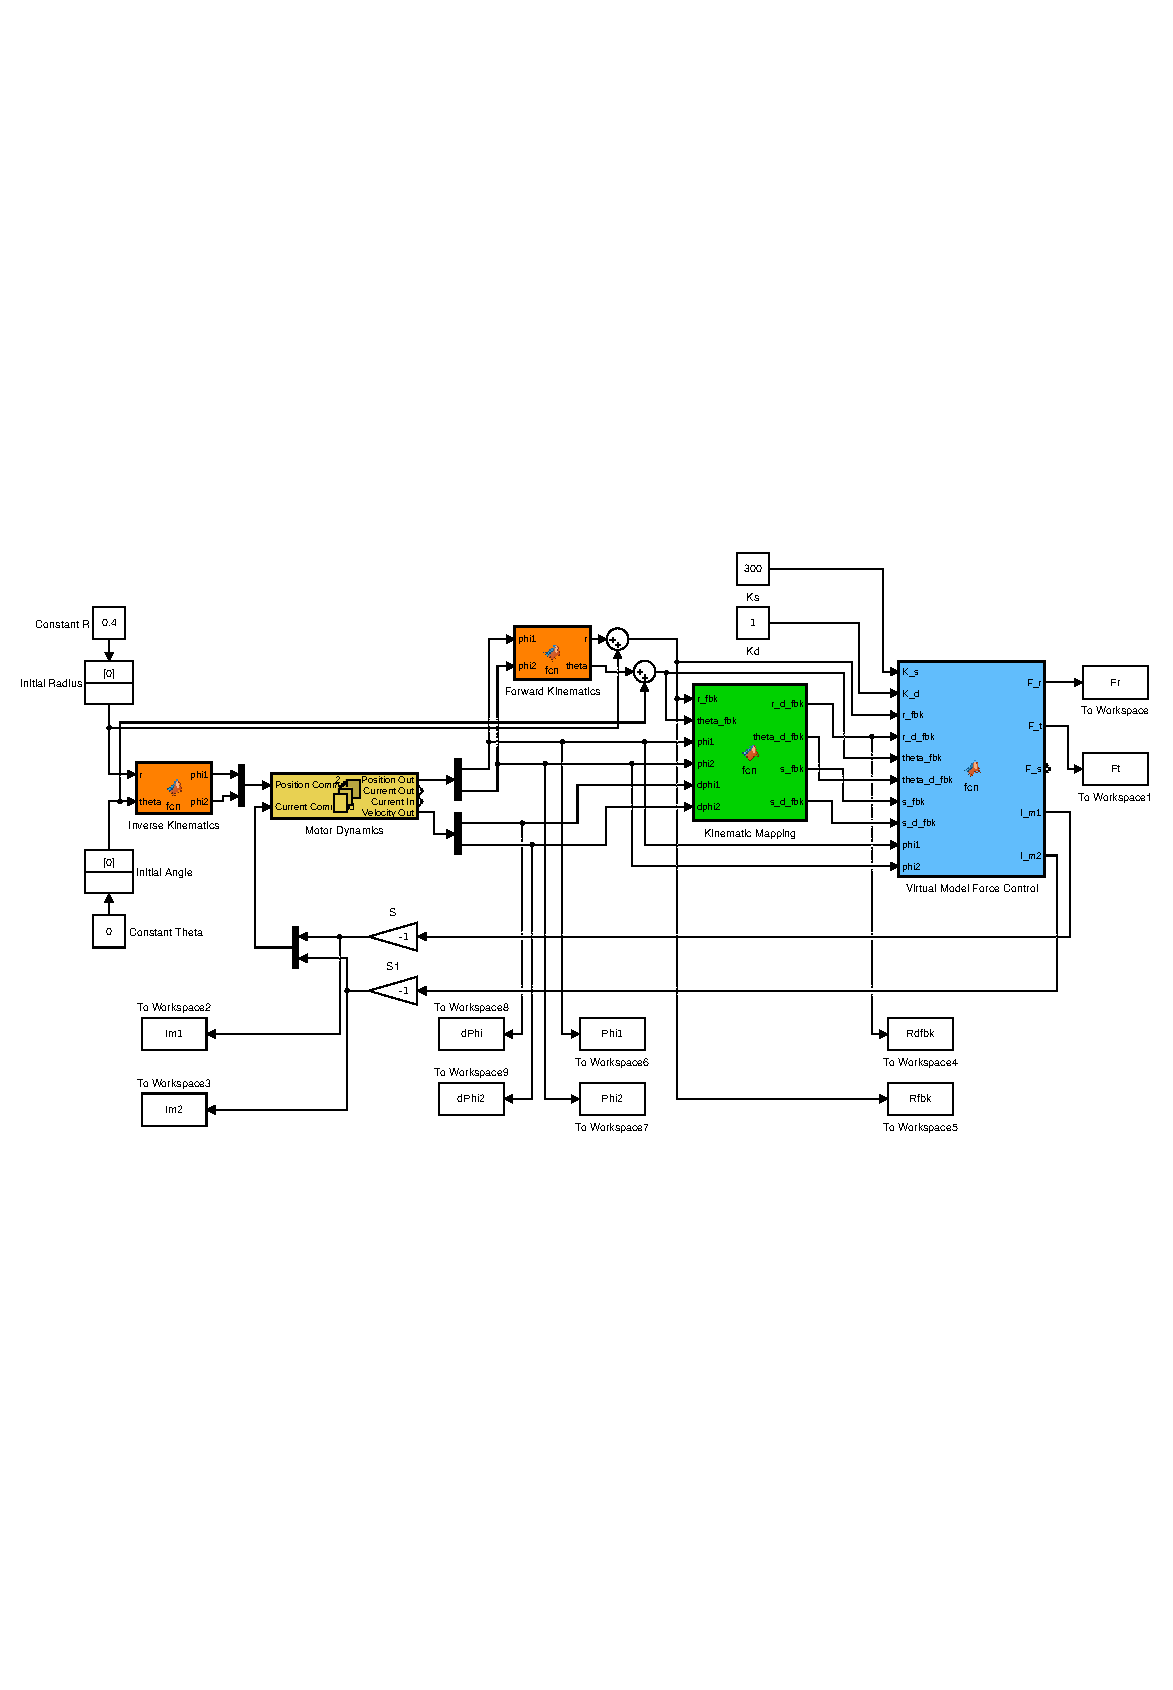
\includegraphics[clip, trim=0cm 8cm 0cm 8cm,width=1\textwidth]{images/simulation/leg-simulation.eps}
\caption{Dynamic and kinematic control simulation model.}
\label{fig:Dynamic and kinematic simulation model}
\end{figure}

\begin{figure}
\centering
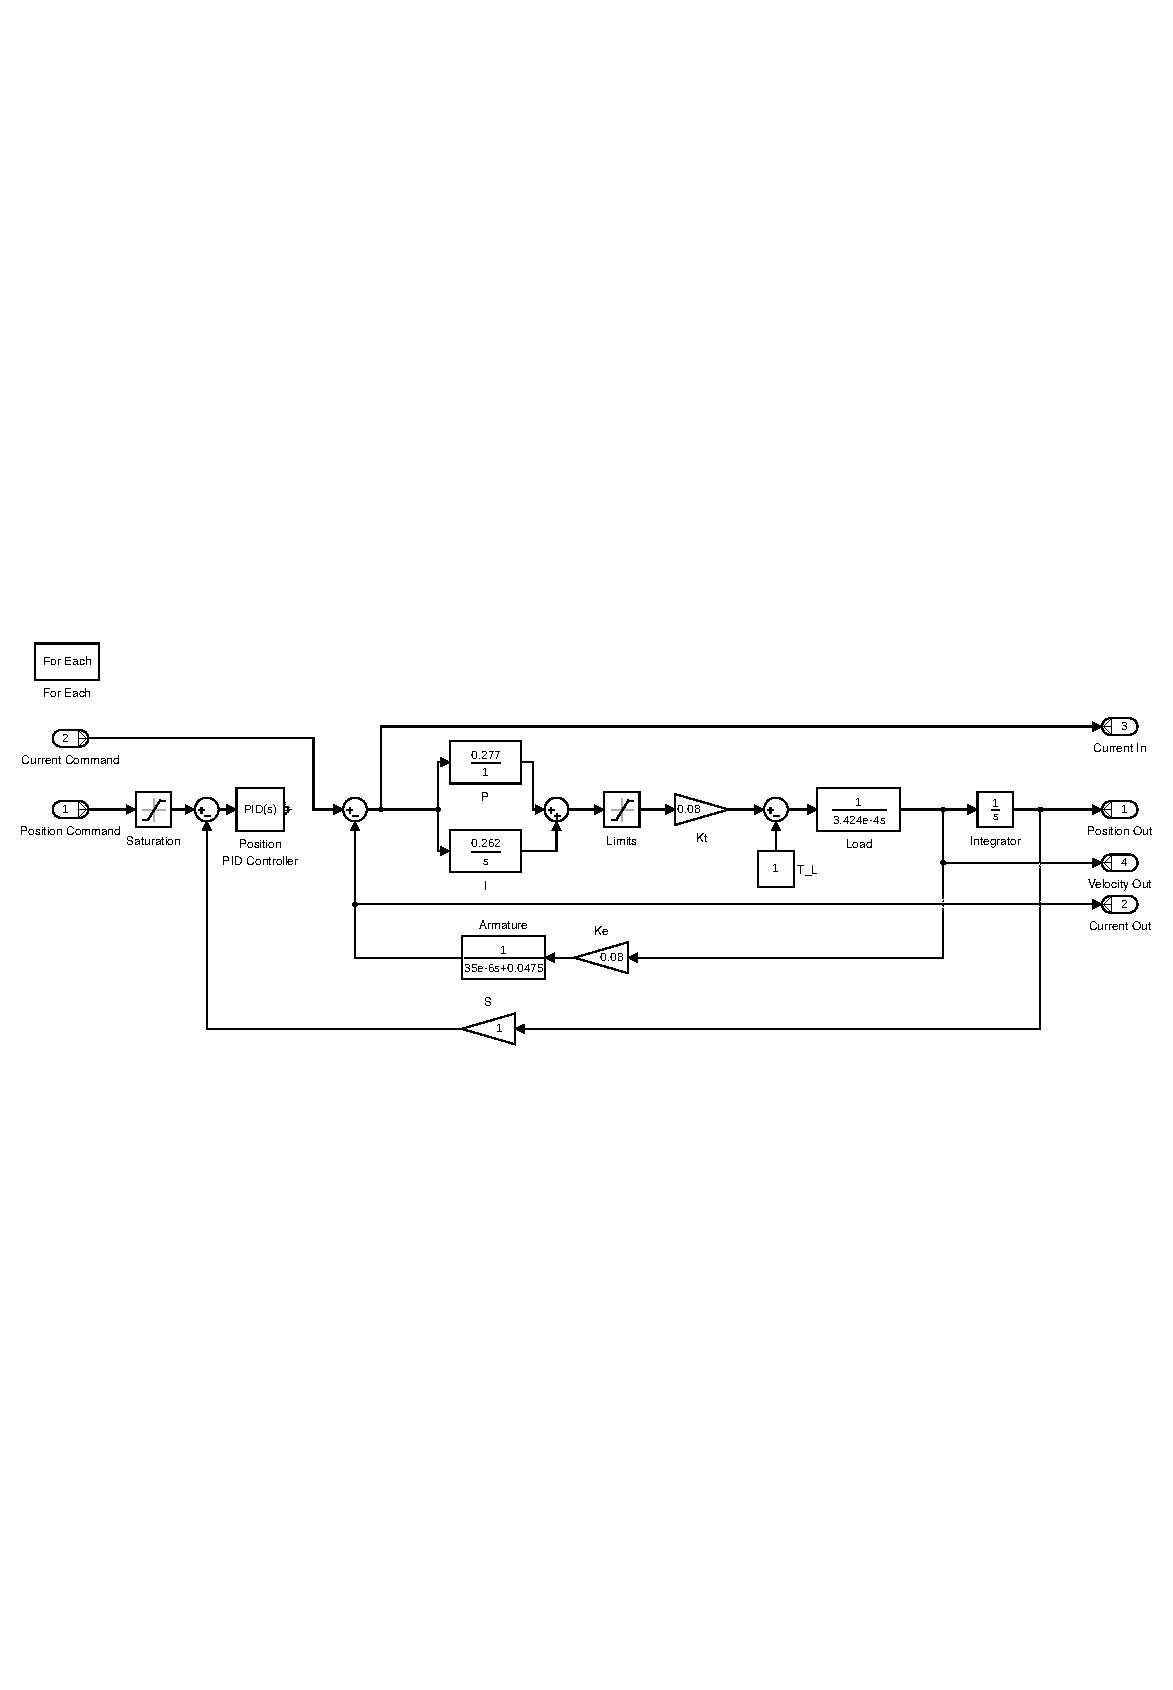
\includegraphics[clip, trim=0cm 10cm 0cm 10cm,width=1\textwidth]{images/simulation/motor-model.eps}
\caption{Motor simulation model.}
\label{fig:Motor simulation model}
\end{figure}

\begin{figure}
\centering
\subfloat[][Radial position.]{
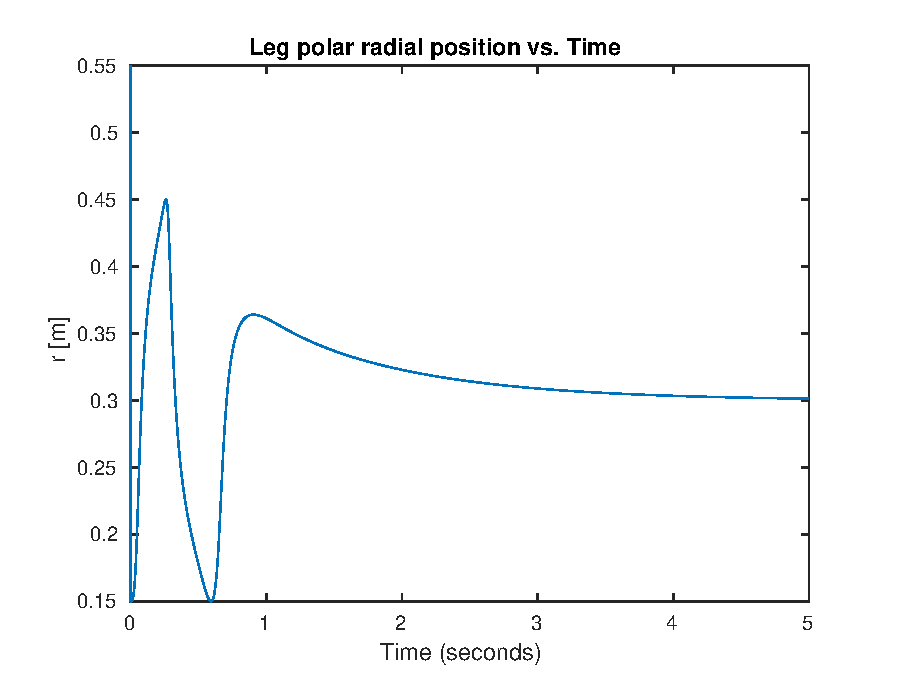
\includegraphics[width=0.5\textwidth]{images/simulation/r.eps}
}
\subfloat[][Radial velocity.]{
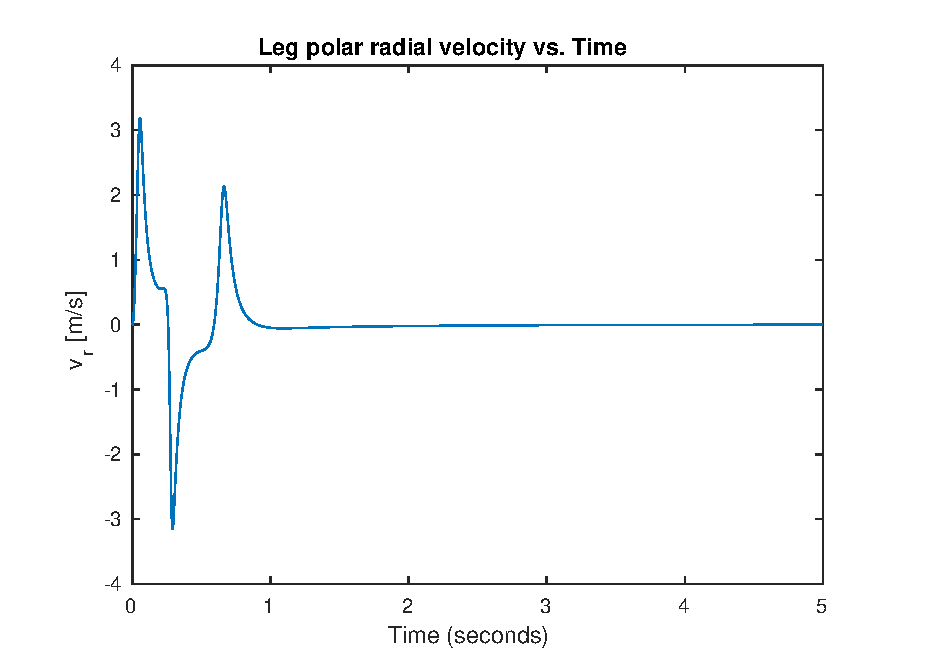
\includegraphics[width=0.5\textwidth]{images/simulation/vr.eps}
}

\subfloat[][Radial force.]{
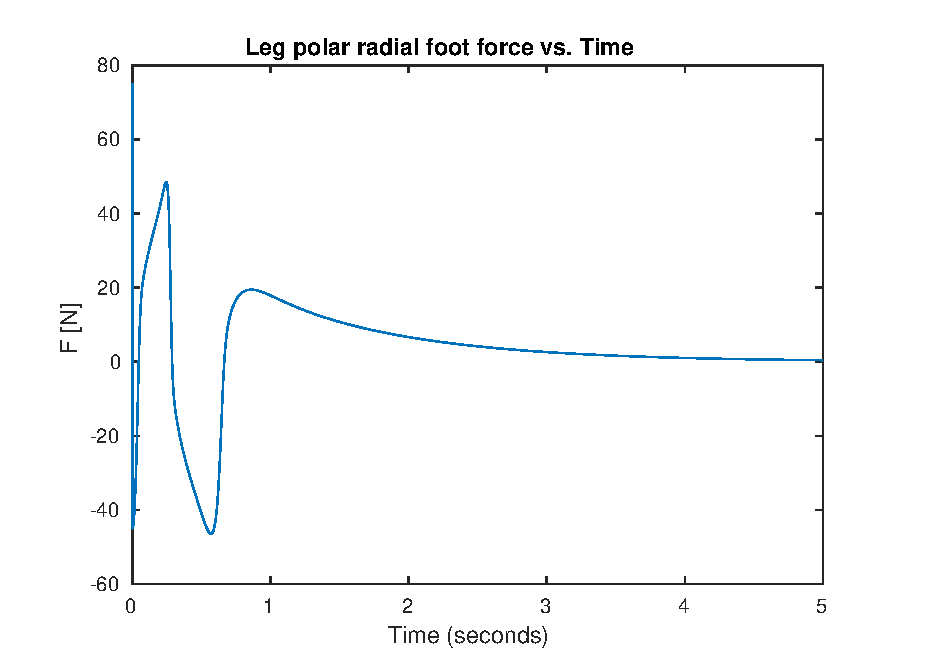
\includegraphics[width=0.5\textwidth]{images/simulation/f.eps}
}
\subfloat[][Motor current.]{
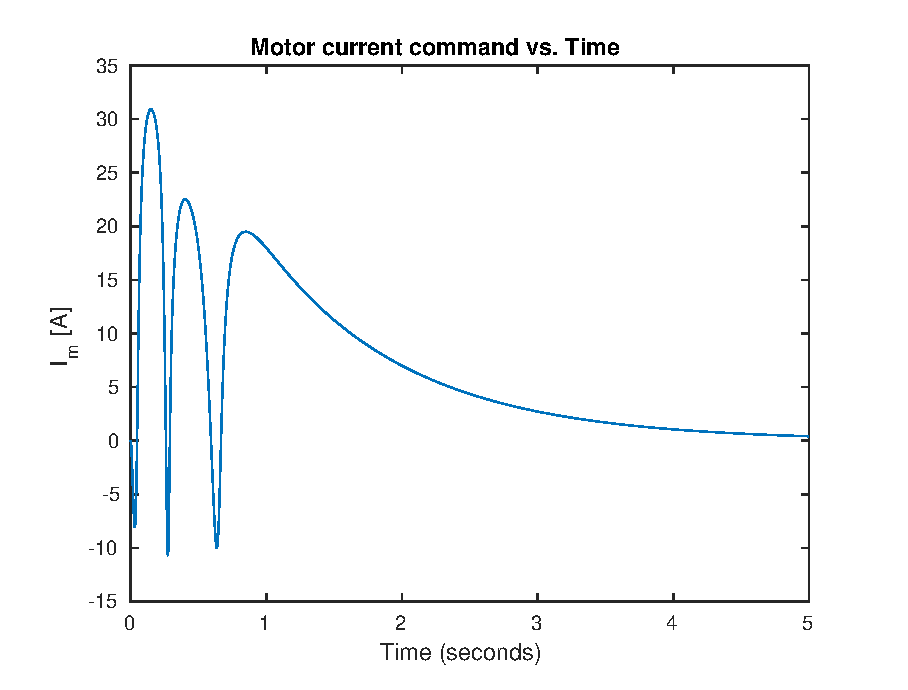
\includegraphics[width=0.5\textwidth]{images/simulation/im.eps}
}
\caption{Control system simulation plots.}
\label{fig:Control system simulation plots}
\end{figure}

